\documentclass{ximera}

 

\usepackage{epsfig}

\graphicspath{
  {./}
  {figures/}
}

\usepackage{morewrites}
\makeatletter
\newcommand\subfile[1]{%
\renewcommand{\input}[1]{}%
\begingroup\skip@preamble\otherinput{#1}\endgroup\par\vspace{\topsep}
\let\input\otherinput}
\makeatother

\newcommand{\includeexercises}{\directlua{dofile("/home/jim/linearAlgebra/laode/exercises.lua")}}

%\newcounter{ccounter}
%\setcounter{ccounter}{1}
%\newcommand{\Chapter}[1]{\setcounter{chapter}{\arabic{ccounter}}\chapter{#1}\addtocounter{ccounter}{1}}

%\newcommand{\section}[1]{\section{#1}\setcounter{thm}{0}\setcounter{equation}{0}}

%\renewcommand{\theequation}{\arabic{chapter}.\arabic{section}.\arabic{equation}}
%\renewcommand{\thefigure}{\arabic{chapter}.\arabic{figure}}
%\renewcommand{\thetable}{\arabic{chapter}.\arabic{table}}

%\newcommand{\Sec}[2]{\section{#1}\markright{\arabic{ccounter}.\arabic{section}.#2}\setcounter{equation}{0}\setcounter{thm}{0}\setcounter{figure}{0}}

\newcommand{\Sec}[2]{\section{#1}}

\setcounter{secnumdepth}{2}
%\setcounter{secnumdepth}{1} 

%\newcounter{THM}
%\renewcommand{\theTHM}{\arabic{chapter}.\arabic{section}}

\newcommand{\trademark}{{R\!\!\!\!\!\bigcirc}}
%\newtheorem{exercise}{}

\newcommand{\dfield}{{\sf dfield9}}
\newcommand{\pplane}{{\sf pplane9}}

\newcommand{\EXER}{\section*{Exercises}}%\vspace*{0.2in}\hrule\small\setcounter{exercise}{0}}
\newcommand{\CEXER}{}%\vspace{0.08in}\begin{center}Computer Exercises\end{center}}
\newcommand{\TEXER}{} %\vspace{0.08in}\begin{center}Hand Exercises\end{center}}
\newcommand{\AEXER}{} %\vspace{0.08in}\begin{center}Hand Exercises\end{center}}

% BADBAD: \newcommand{\Bbb}{\bf}

\newcommand{\R}{\mbox{$\Bbb{R}$}}
\newcommand{\C}{\mbox{$\Bbb{C}$}}
\newcommand{\Z}{\mbox{$\Bbb{Z}$}}
\newcommand{\N}{\mbox{$\Bbb{N}$}}
\newcommand{\D}{\mbox{{\bf D}}}
\usepackage{amssymb}
%\newcommand{\qed}{\hfill\mbox{\raggedright$\square$} \vspace{1ex}}
%\newcommand{\proof}{\noindent {\bf Proof:} \hspace{0.1in}}

\newcommand{\setmin}{\;\mbox{--}\;}
\newcommand{\Matlab}{{M\small{AT\-LAB}} }
\newcommand{\Matlabp}{{M\small{AT\-LAB}}}
\newcommand{\computer}{\Matlab Instructions}
\newcommand{\half}{\mbox{$\frac{1}{2}$}}
\newcommand{\compose}{\raisebox{.15ex}{\mbox{{\scriptsize$\circ$}}}}
\newcommand{\AND}{\quad\mbox{and}\quad}
\newcommand{\vect}[2]{\left(\begin{array}{c} #1_1 \\ \vdots \\
 #1_{#2}\end{array}\right)}
\newcommand{\mattwo}[4]{\left(\begin{array}{rr} #1 & #2\\ #3
&#4\end{array}\right)}
\newcommand{\mattwoc}[4]{\left(\begin{array}{cc} #1 & #2\\ #3
&#4\end{array}\right)}
\newcommand{\vectwo}[2]{\left(\begin{array}{r} #1 \\ #2\end{array}\right)}
\newcommand{\vectwoc}[2]{\left(\begin{array}{c} #1 \\ #2\end{array}\right)}

\newcommand{\ignore}[1]{}


\newcommand{\inv}{^{-1}}
\newcommand{\CC}{{\cal C}}
\newcommand{\CCone}{\CC^1}
\newcommand{\Span}{{\rm span}}
\newcommand{\rank}{{\rm rank}}
\newcommand{\trace}{{\rm tr}}
\newcommand{\RE}{{\rm Re}}
\newcommand{\IM}{{\rm Im}}
\newcommand{\nulls}{{\rm null\;space}}

\newcommand{\dps}{\displaystyle}
\newcommand{\arraystart}{\renewcommand{\arraystretch}{1.8}}
\newcommand{\arrayfinish}{\renewcommand{\arraystretch}{1.2}}
\newcommand{\Start}[1]{\vspace{0.08in}\noindent {\bf Section~\ref{#1}}}
\newcommand{\exer}[1]{\noindent {\bf \ref{#1}}}
\newcommand{\ans}{}
\newcommand{\matthree}[9]{\left(\begin{array}{rrr} #1 & #2 & #3 \\ #4 & #5 & #6
\\ #7 & #8 & #9\end{array}\right)}
\newcommand{\cvectwo}[2]{\left(\begin{array}{c} #1 \\ #2\end{array}\right)}
\newcommand{\cmatthree}[9]{\left(\begin{array}{ccc} #1 & #2 & #3 \\ #4 & #5 &
#6 \\ #7 & #8 & #9\end{array}\right)}
\newcommand{\vecthree}[3]{\left(\begin{array}{r} #1 \\ #2 \\
#3\end{array}\right)}
\newcommand{\cvecthree}[3]{\left(\begin{array}{c} #1 \\ #2 \\
#3\end{array}\right)}
\newcommand{\cmattwo}[4]{\left(\begin{array}{cc} #1 & #2\\ #3
&#4\end{array}\right)}

\newcommand{\Matrix}[1]{\ensuremath{\left(\begin{array}{rrrrrrrrrrrrrrrrrr} #1 \end{array}\right)}}

\newcommand{\Matrixc}[1]{\ensuremath{\left(\begin{array}{cccccccccccc} #1 \end{array}\right)}}



\renewcommand{\labelenumi}{\theenumi)}
\newenvironment{enumeratea}%
{\begingroup
 \renewcommand{\theenumi}{\alph{enumi}}
 \renewcommand{\labelenumi}{(\theenumi)}
 \begin{enumerate}}
 {\end{enumerate}\endgroup}



\newcounter{help}
\renewcommand{\thehelp}{\thesection.\arabic{equation}}

%\newenvironment{equation*}%
%{\renewcommand\endequation{\eqno (\theequation)* $$}%
%   \begin{equation}}%
%   {\end{equation}\renewcommand\endequation{\eqno \@eqnnum
%$$\global\@ignoretrue}}

%\input{psfig.tex}

\author{Martin Golubitsky and Michael Dellnitz}

%\newenvironment{matlabEquation}%
%{\renewcommand\endequation{\eqno (\theequation*) $$}%
%   \begin{equation}}%
%   {\end{equation}\renewcommand\endequation{\eqno \@eqnnum
% $$\global\@ignoretrue}}

\newcommand{\soln}{\textbf{Solution:} }
\newcommand{\exercap}[1]{\centerline{Figure~\ref{#1}}}
\newcommand{\exercaptwo}[1]{\centerline{Figure~\ref{#1}a\hspace{2.1in}
Figure~\ref{#1}b}}
\newcommand{\exercapthree}[1]{\centerline{Figure~\ref{#1}a\hspace{1.2in}
Figure~\ref{#1}b\hspace{1.2in}Figure~\ref{#1}c}}
\newcommand{\para}{\hspace{0.4in}}

\renewenvironment{solution}{\suppress}{\endsuppress}

\ifxake
\newenvironment{matlabEquation}{\begin{equation}}{\end{equation}}
\else
\newenvironment{matlabEquation}%
{\let\oldtheequation\theequation\renewcommand{\theequation}{\oldtheequation*}\begin{equation}}%
  {\end{equation}\let\theequation\oldtheequation}
\fi

\makeatother


\title{A Single Differential Equation}

\begin{document}
\begin{abstract}
\end{abstract}
\maketitle

  \label{S:growthmodels}

Algebraic operations such as addition and multiplication are
performed on numbers while the calculus operations of
differentiation and integration are performed on functions.
Thus algebraic equations (such as $x^2=9$) are solved for
numbers ($x=\pm 3$) while differential (and integral) equations
are solved for functions.

In Chapter~\ref{lineq} we discussed how to solve systems of
linear equations, such as
\begin{eqnarray*}
x_1 + x_2 & = & 2 \\
x_1 - x_2 & = & 4
\end{eqnarray*}
for numbers
\[
x_1=3 \quad \mbox{ and } \quad x_2=-1,
\]
while in this chapter we discuss how to solve some systems of
differential equations for functions.

Solving a single linear equation in one unknown $x$ is a simple
task.  For example, solve
\[
2x = 4
\]
for $x=2$.  Solving a single differential equation in one unknown function
$x(t)$ is far from trivial.

\subsubsection*{Integral Calculus as a Differential Equation}
\index{integral calculus}

Mathematically, the simplest type of differential equation is:
\begin{equation} \label{e:intcalc}
\dps\frac{dx}{dt}(t) = f(t)
\end{equation}
where $f$ is some continuous function.  In words, this equation asks us
to find all functions $x(t)$ whose derivative is $f(t)$.  The fundamental
theorem of calculus tells us the answer: $x(t)$ is an antiderivative of
$f(t)$.  Thus to find all solutions, we just integrate both sides of
\eqref{e:intcalc} with respect to $t$.  Formally, using indefinite integrals, 
\begin{equation}  \label{E:integrate}
\int \frac{dx}{dt}(t)dt = \int f(t)dt + C,
\end{equation}
where $C$ is an arbitrary constant.  (It is tempting to put a constant of
integration on both sides of \eqref{E:integrate}, but two constants are not 
needed, as we can just combine both constants on the right hand side of
this equation.)   Since the indefinite integral of $dx/dt$ is just the
function $x(t)$, we have 
\begin{equation}  \label{e:intcalcsoln}
x(t) = \int f(\tau) d\tau + C.
\end{equation}
In particular, finding closed form solutions to differential equations
of the type \eqref{e:intcalc} is equivalent to finding all definite
integrals of the function $f(t)$.  Indeed, to find closed form solutions 
to differential equations like \eqref{e:intcalc} we need to know all of the 
techniques of integration from integral calculus.

We note that if $x(t)$ is a real-valued function of $t$, then we denote the 
derivative of $x$ with respect to $t$ using the following
\[
\frac{dx}{dt}\qquad \dot{x} \qquad x'
\]
all of which are standard notations for the derivative.


\subsubsection*{Initial Conditions and the Role of the Integration Constant 
$C$}

Equation \eqref{e:intcalcsoln} tells us that there are an infinite number of
solutions to the differential equation \eqref{e:intcalc}, each one
corresponding to a different choice of the constant $C$.  To understand how
to interpret the constant $C$, consider the example
\[
\dps\frac{dx}{dt}(t) = \cos t.
\]
Using \eqref{e:intcalcsoln} we see that the answer is
\[
x(t) = \int \cos\tau d\tau  + C = \sin t + C.
\]
Note that 
\[
x(0) = \sin(0) + C = C.
\]
Thus, the constant $C$ represents an {\em initial condition\/} for the  
differential equation.  We will return to the discussion of initial 
conditions several times in this chapter.

See Exercise~\ref{c3.1.7} for a more interesting example of this type of
differential equation.

\subsubsection*{Solutions to Differential Equations are Functions}

Consider the differential equation \index{differential equation}
\begin{equation} \label{E:verify}
\frac{dx}{dt}(t) = tx(t).
\end{equation}
Are the functions
\[
x_1(t) = t^2 \AND x_2(t) = e^{t^2/2}
\]
solutions to the differential equation \eqref{E:verify}?

To test whether or not the function $x_1(t)$ is a solution, we compute
the left and right hand sides of \eqref{E:verify}:
\begin{eqnarray*}
{\rm LHS:} & \frac{d}{dt}x_1(t) & = 2t\\
{\rm RHS:} &  tx_1(t) & = t^3.
\end{eqnarray*}
Since the left and right hand sides are unequal, the function $x_1(t)$
is not a solution to \eqref{E:verify}.

To test whether or not the function $x_2(t)$ is a solution, we again
compute the left and right hand sides of \eqref{E:verify}:
\begin{eqnarray*}
{\rm LHS:} & \frac{d}{dt}x_2(t) & = te^{t^2/2}\\
{\rm RHS:} &  tx_2(t) & = te^{t^2/2}.
\end{eqnarray*}
Since the left and right hand sides are equal, the function $x_2(t)$
is a solution to \eqref{E:verify}.

Note that we have not discussed how we knew that the function $x_2(t)$
is a solution to \eqref{E:verify}.  For the most part, the issue of how
one finds solutions to a differential equation will be discussed in later
chapters, though we do determine solutions to a very important equation next.

\subsubsection*{The Linear Differential Equation of Growth and Decay}

The real subject of differential equations begins when the function $f$
on the right hand side of \eqref{e:intcalc} depends explicitly on the
function $x$, and the simplest such differential equation is:
\[
\frac{dx}{dt}(t) = x(t).
\]
Using results from calculus, we can solve this equation; indeed,
we can solve the slightly more complicated equation
\begin{equation}  \label{lin1}
\frac{dx}{dt}(t) = \lambda x(t),
\end{equation}
where $\lambda\in\R$ is a constant.  The differential equation \eqref{lin1} is 
{\em linear\/} since $x(t)$ appears by itself on the right hand side.  
Moreover, \eqref{lin1} is {\em homogeneous\/} since the constant function 
$x(t)=0$ is a solution.


In words \eqref{lin1} asks: For which functions $x(t)$ is the
derivative of $x(t)$ a scalar multiple of $x(t)$.  The function
\[
x(t)=e^{\lambda t}
\]
is such a function, since
\[
\frac{dx}{dt}(t) = \frac{d}{dt}e^{\lambda t} =
\lambda e^{\lambda t} = \lambda x(t).
\]
More generally, the function
\begin{equation} \label{soln1}
x(t) = K e^{\lambda t}
\end{equation}
is a solution to \eqref{lin1} for any real constant $K$.  We claim
that the functions \eqref{soln1} list all (differentiable)
functions that solve \eqref{lin1}.

To verify this claim, we let $x(t)$ be a solution to \eqref{lin1}
and show that the ratio 
\[
\frac{x(t)}{e^{\lambda t}} = x(t)e^{-\lambda t}
\]
is a constant (independent of $t$).  Using the product rule 
\index{product rule} and \eqref{lin1}, compute
\begin{eqnarray*}
\frac{d}{dt}\left[x(t)e^{-\lambda t}\right] & = &
\frac{d}{dt}\left(x(t)\right) e^{-\lambda t} +
x(t)\frac{d}{dt}\left(e^{-\lambda t}\right) \\
& = &
(\lambda x(t)) e^{-\lambda t} + x(t)(-\lambda e^{-\lambda t}) \\
& = & 0.
\end{eqnarray*}
Now recall that the only functions whose derivatives are
identically zero are the constant functions.  Thus,
\[
x(t) e^{-\lambda t} = K
\]
for some constant $K\in\R$.  Hence $x(t)$ has the form
\eqref{soln1}, as claimed.

Next, we discuss the role of the constant $K$.  We have written
the function as $x(t)$, and we have meant the reader to think of
the variable $t$ as time.  Thus $x(0)$ is the initial value of
the function $x(t)$ at time $t=0$; we say that $x(0)$ is the
{\em initial value\/}\index{initial value problem} of $x(t)$.
From \eqref{soln1} we see that
\[
x(0) = K,
\]
and that $K$ is the initial value of the solution of \eqref{lin1}.
Henceforth, we write $K$ as $x_0$ so that the notation calls
attention to the special meaning of this constant.

By deriving \eqref{soln1} we have proved:
\begin{theorem}  \label{T:singleeqn}
There is a unique solution to the {\em initial value problem\/}
\index{initial value problem}
\arraystart
\begin{equation} \label{ivp1}
\begin{array}{rcl}
\dps \frac{dx}{dt}(t) & = & \lambda x(t) \\
x(0) & = & x_0.
\end{array}
\end{equation}
\arrayfinish
That solution is
\[
x(t) = x_0e^{\lambda t}.
\]
\end{theorem}

As a consequence of Theorem~\ref{T:singleeqn} we see that there
is a qualitative difference in the behavior of solutions to
\eqref{ivp1} depending on whether $\lambda>0$ or $\lambda<0$.
Suppose that $x_0>0$.  Then
\begin{equation}  \label{explimits}
\lim_{t\to\infty} x(t) = \lim_{t\to\infty} x_0e^{\lambda t} =\left\{
\begin{array}{rl} +\infty & \quad\lambda>0 \\ 0 & \quad\lambda<0 . \end{array}
\right.
\end{equation}
When $\lambda>0$ we say that the solution has {\em exponential
growth\/}\index{exponential!growth} and when $\lambda< 0$ we say
that the solution has {\em exponential decay\/}
\index{exponential!decay}.  In either case, however, the
number $\lambda$ is called the {\em growth rate\/}\index{growth
rate}.  We can visualize this discussion by graphing the
solutions in \Matlabp.

Suppose we set $x_0=1$ and $\lambda=\pm 0.5$.  Type
\begin{verbatim}
x0 = 1;
lambda = 0.5;
t = linspace(-1,4,100);
x = x0*exp(lambda*t);
plot(t,x)
hold on
xlabel('t')
ylabel('x')
lambda = -0.5;
x = x0*exp(lambda*t);
plot(t,x)
\end{verbatim}
The result of this calculation is shown in
Figure~\ref{graph_labelfig}.  In this way we can actually see
the difference between exponential growth ($\lambda=0.5$) and
exponential decay ($\lambda=-0.5$), as discussed in
\eqref{explimits}.

\begin{figure}[htb]
     \centerline{%
     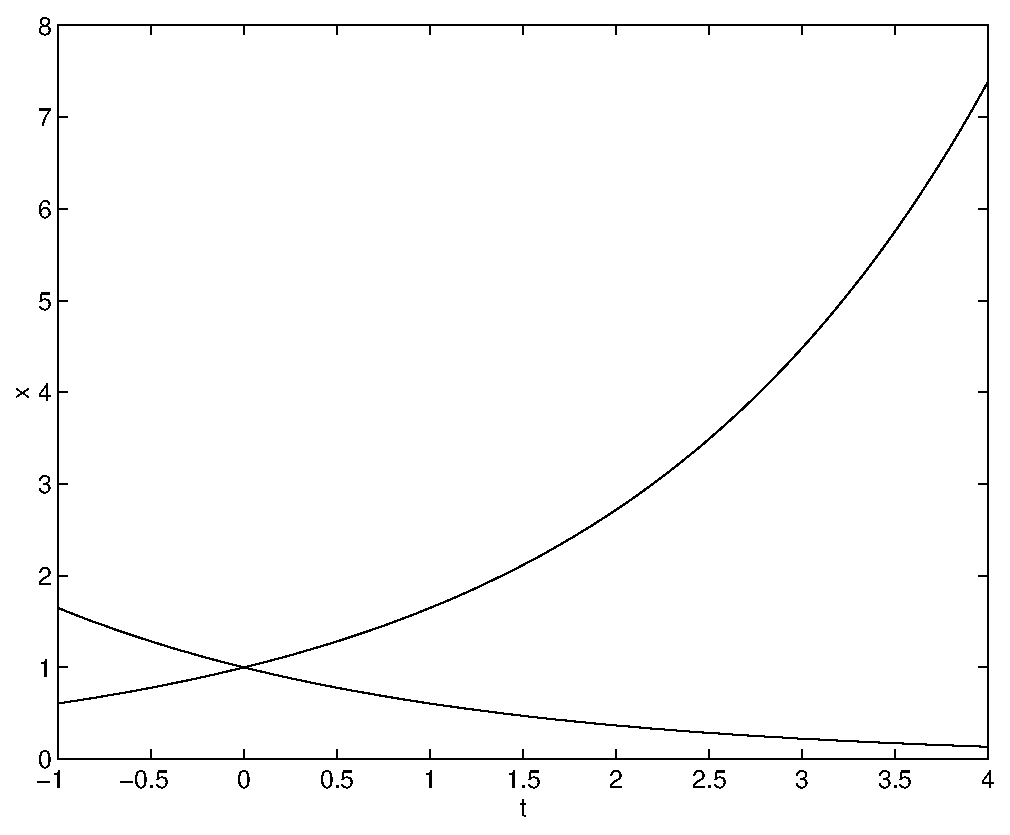
\psfig{file=../figures/graph1.eps,width=3.5in}}
     \caption{Solutions of \protect\eqref{lin1}
              for $t\in [-1,4]$, $x_0=1$ and $\lambda=\pm 0.5$.}
     \label{graph_labelfig}
\end{figure}

\ignore{
  \subsubsection*{The Inhomogeneous Linear Differential Equation}

It follows from \eqref{explimits} that solutions to the linear homogeneous
differential equation \eqref{ivp1} are either unbounded as $t\to \infty$ or 
they approach zero.  Now we consider an inhomogeneous differential 
equation and show that solutions can approach fixed values for increasing 
$t$ that are neither zero nor infinity.

As an example, consider the linear differential equation
\begin{equation} \label{E:ivp2}
\frac{dx}{dt} = -2x-6.
\end{equation}
Observe that $x(t)=0$ is not a solution of \eqref{E:ivp2} and therefore
that \eqref{E:ivp2} is {\em inhomogeneous}.  It is easy to verify, however, 
that the constant function $x(t)=-3$ is a solution.

Equation~\eqref{E:ivp2} can be solved by introducing a new function that 
transforms \eqref{E:ivp2} into a homogeneous equation.  Let
\[
y(t) = x(t) + 3,
\]
and compute
\[
\frac{dy}{dt} = \frac{dx}{dt} = -2x-6 = -2y.
\]

Using Theorem~\ref{T:singleeqn}, it follows that $y(t)$ has the form
\[
y(t) = y_0e^{-2t}.
\]
Therefore
\[
x(t) =  y_0e^{-2t}-3
\]
is a solution of \eqref{E:ivp2} for every constant $y_0$.  Moreover, 
\[
\lim_{t\to\infty} x(t) = \lim_{t\to\infty} y_0e^{-2t} -3=-3,
\]
which is neither zero nor infinity.

Any equation of the form
\begin{equation} \label{ivp2}
\frac{dx}{dt}(t)  = \lambda x(t) +\rho
\end{equation}
can be solved in a similar fashion.  Just set 
\[
y(t) = x(t) + \frac{\rho}{\lambda}.
\]
It follows from \eqref{ivp2} that
\[
\frac{dy}{dt} = \frac{dx}{dt} = \lambda x(t) +\rho =
\lambda\left( y(t)-\frac{\rho}{\lambda}\right) +\rho = \lambda y(t).
\]
Theorem~\ref{T:singleeqn} implies that $y(t) = y_0e^{\lambda t}$ for some 
constant $y_0$ and
\[
x(t) = y_0e^{\lambda t} - \frac{\rho}{\lambda}.
\]
Note that the limit of $x(t)$ as $t\to\infty$ is $-\rho/\lambda$ when 
$\lambda<0$.
}


\subsection*{Some Examples of \protect\eqref{ivp1}}

Even though the differential equation \eqref{lin1} is one of the
simplest differential equations, it still has some use in applications.
We present two here: compound interest and population dynamics.

\subsubsection*{Compound Interest} \index{compound interest}

Banks pay interest on an account in the following way.  At the
end of each day, the bank determines the interest rate $r_{day}$ for
that day, checks the principal $P$ in the account, and then
deposits an additional $r_{day}P$.  So the next day the principal in
this account is $(1+r_{day})P$.  Note that if $r$ denotes the
interest rate per year, then $r_{day} = r/365$.  Of course, a day
is just a convenient measure for elapsed time.  Before computers
were prevalent, banks paid interest yearly or quarterly or monthly
or, in a few cases, even weekly, depending on the particular bank rules.

Observe that the more frequently interest is paid, the more
money is earned. For example, if interest is paid only once at
the end of a year, then the money in the account at the end of
the year is $(1+r)P$, and the amount $rP$ is called {\em simple
interest\/}.  But if interest is paid twice a year, then the principal
at the end of six months will be $(1+\frac{r}{2})P$, and the principal
at the end of the year will be $(1+\frac{r}{2})^2P$.  Since
\[
\left(1+\frac{r}{2}\right)^2 = 1+r+\frac{1}{4}r^2 > 1+r,
\]
there is more money in the account at the end of the
year if the interest is compounded semiannually rather than
annually.  But how much is the difference and what is the
maximum earning potential?

While making the calculation in the previous paragraph, we
implicitly made a number of simplifying assumptions.  In
particular, we assumed
\begin{itemize}
\item	an initial principal $P_0$ is deposited in the bank on January 1,
\item	the money is not withdrawn for one year,
\item	no new money is deposited in that account during the year,
\item	the yearly interest rate $r$ remains constant throughout
	the year, and
\item	interest is added to the account $N$ times during the year.
\end{itemize}
In this {\em model\/}, simple interest corresponds to $N=1$, compound monthly
interest to $N=12$, and compound daily interest to $N=365$.

We first answer the question: How much money is in this account after
one year?  After one time unit of $\frac{1}{N}$ year, the amount of
money in the account is
\[
Q_1 = \left(1+\frac{r}{N}\right)P_0.
\]
The interest rate in each time period is $\frac{r}{N}$,
the yearly rate $r$ divided by the number of time periods $N$.  Here
we have used the assumption that the interest rate remains constant
throughout the year.  After two time units, the principal is:
\[
Q_2 = \left(1+\frac{r}{N}\right)Q_1 = \left(1+\frac{r}{N}\right)^2P_0,
\]
and at the end of the year (that is, after $N$ time periods)
\begin{equation} \label{compint}
Q_N = \left(1+\frac{r}{N}\right)^N P_0.
\end{equation}
Here we have used the assumption that money is neither deposited nor
withdrawn from our account.   Note that $Q_N$ is the amount of money
in the bank after {\bf one} year assuming that interest has been
compounded $N$ (equally spaced) times during that year, and the effective
interest rate when compounding $N$ times is:
\[
\left(1+\frac{r}{N}\right)^N - 1.
\]

For the curious, we can write a program in \Matlab to compute
\eqref{compint}.  Suppose we assume that the initial deposit $P_0=\$1,000$,
the simple interest rate is $6\%$ per year, and the interest payments
are made monthly. In \Matlab type
\begin{verbatim}
N  = 12;
P0 = 1000;
r  = 0.06;
QN = (1 + r/N)^N*P0
\end{verbatim}
The answer is $QN=\$1,061.68$, and the {\em effective\/}
interest rate for monthly payments is $6.16778\%$.  For daily
interest payments $N=365$, the answer is $QN=\$1,061.83$, and
the effective interest rate is $6.18313\%$.

To find the maximum effective interest, we ask the bank to compound interest
continuously; that is, we ask the bank to compute
\[
\lim_{N\to\infty} \left(1 + \frac{r}{N}\right)^N.
\]
We compute this limit using differential equations.  The concept of
continuous interest is rephrased as follows.  Let $P(t)$ be the
principal at time $t$, where $t$ is measured in units of years.
Suppose that we assume that interest is compounded $N$ times during
the year.  The length of time in each compounding period is
\[
\Delta t = \frac{1}{N},
\]
and the change in principal during that time period is
\[
\Delta P = \frac{r}{N} P = rP\Delta t.
\]
It follows that
\[
\frac{\Delta P}{\Delta t} = rP,
\]
and, on taking the limit $\Delta t \to 0$, we have the differential equation
\[
\frac{dP}{dt}(t) = rP(t).
\]

Since $P(0)=P_0$ the solution of the initial value problem given
in Theorem~\ref{T:singleeqn} shows that
\[
P(t) = P_0 e^{rt}.
\]
After one year ($t=1$) we find that
\[
P(1) =  e^r P_0.
\]
Note that
\[
P(1) = \lim_{N\to\infty} Q_N,
\]
and we have thus verified that
\[
 \lim_{N\to\infty} \left(1 + \frac{r}{N}\right)^N = e^r.
\]
Thus the maximum effective interest rate is $e^r-1$.  When $r=6\%$
the maximum effective interest rate is $6.18365\%$.


\subsubsection*{An Example from Population Dynamics}
\index{population dynamics}

To provide a second interpretation of the constant $\lambda$ in
\eqref{lin1}, we discuss a simplified model for population dynamics.
Let $p(t)$ be the size of a population of a certain species at
time $t$ and let $r$ be the rate at which the population $p$ is
changing at time $t$.  In general, $r$ depends on the time $t$
and is a complicated function of birth and death rates and of
immigration and emigration, as well as of other factors.
Indeed, the rate $r$ may well depend
on the size of the population itself.  (Overcrowding can be
modeled by assuming that the death rate increases with the size
of the population.) These population models assume that the
rate of change in the size of the population $dp/dt$ is given by
\begin{equation}  \label{pop_model}
        \frac{dp}{dt}(t) = r p(t),
\end{equation}
they just differ on the precise form of $r$.  In general, the
rate $r$ will depend on the size of the population $p$ as well
as the time $t$, that is, $r$ is a function $r(p,t)$.

The simplest population model\index{population model} --- which
we now assume --- is the
one in which $r$ is assumed to be constant.  Then equation
\eqref{pop_model} is identical to \eqref{lin1} after identifying $p$
with $x$ and $r$ with $\lambda$.  Hence we may interpret $r$ as
the growth rate for the population.  The form of the solution in
\eqref{soln1} shows that the size of a population grows
exponentially if $r>0$ and decays exponentially if $r<0$.

The mathematical description of this simplest population model
shows that the assumption of a constant growth rate leads to
exponential growth (or exponential decay).  Is this realistic?
Surely, no population will grow exponentially for all time, and
other factors, such as limited living space, have to be taken
into account.  On the other hand, exponential growth describes
well the growth in human population during much of human
history.  So this model, though surely oversimplified, gives
some insight into population growth.

\EXER

\includeexercises


\end{document}
